% =====================================================================
%  SNIPPETS – Kopiervorlagen für den Laborbericht (MCI-Formalkriterien)
%
%  Diese Datei ist eigenständig kompilierbar (gleiche Klasse wie main.tex),
%  damit man sieht, wie jeder Baustein aussieht. Zum Verwenden den Block
%  zwischen  %>>>  und  %<<<  kopieren, in ein Kapitel einfügen, anpassen.
%
%  Voraussetzungen in main.tex (Präambel), falls ein Block sie braucht:
%    \usepackage{booktabs}             % Tabellen (Abschnitt 4)
%    \usepackage{pgfplots}             % Diagramme direkt in LaTeX (Abschnitt 5.4)
%    \pgfplotsset{compat=1.18}
%  Die Platzhalterbilder (example-image) stammen aus dem Paket mwe –
%  im echten Bericht durch eigene Dateien aus img/ ersetzen.
% =====================================================================
\documentclass[state=Report]{mcidoc}
\usepackage{tabularx}
\usepackage{booktabs}
\usepackage{pgfplots}
\pgfplotsset{compat=1.18}
\usepackage[autostyle=true]{csquotes}            % englische Anführungszeichen
\usepackage[backend=biber, style=ieee]{biblatex}
\addbibresource{Vorlagen.bib}
\sisetup{locale = UK, uncertainty-mode = separate} % Unsicherheit mit ± (M031)

\SetMCI{Language = EN,
    Degree = BSc,
    Title = {Snippets},
    StudentID = {62200181, 12313575},
    Student/Name = {Mathias Außerlechner, Benedikt Motzet},
    Report/Supervisor/Name = {FH-Prof. Yeongmi Kim, PhD},
    Report/Cohort = {BA-MECH-24-4C},
    Report/Lecture = {Control Engineering \uppercase\expandafter{\romannumeral 2}},
    Report/Date = {\today},
    Report/Mode = Lab,
    Report/ToC/Primary = set,
    Report/ToC/Figures = set,
    Report/ToC/Tables  = set,
}

\begin{document}

% #####################################################################
\chapter{Text and Wording}
% #####################################################################

\section{Style (M019, M022)}
%>>> Passiv + Präsens, keine Ich-/Wir-Form, kein Fettdruck/Unterstreichen
The step response of the motor is recorded with an oscilloscope. The
controller parameters are determined with the method described in
Section~\ref{sec:eq}. Important terms are \emph{emphasised} in italics, not
underlined.
%<<<

\section{Lists (M018)}
%>>> Immer dieselbe Aufzählungsart verwenden
\begin{itemize}
  \item first item,
  \item second item.
\end{itemize}
\begin{enumerate}
  \item The supply voltage is switched on.
  \item The reference signal is applied.
\end{enumerate}
%<<<

\section{Cross-References (Festlegung)}
%>>> Einheitliche Verweise: Figure~ / Table~ / Equation~ / Chapter~ / Section~
The measured data are listed in Table~\ref{tab:simple} and plotted in
Figure~\ref{fig:plot}. The model follows from Equation~\eqref{eq:pt1}
(see Chapter~\ref{ch:eq}).
%<<<

% #####################################################################
\chapter{Numbers and Units}
% #####################################################################
%>>> siunitx: Zahl + Einheit immer mit \qty / \num / \unit (M023–M031)
\begin{itemize}
  \item Quantity with unit: \qty{12.5}{\volt}, \qty{3.2}{\milli\ampere},
        \qty{50}{\milli\metre}
  \item Composite unit: \qty{1.5}{\metre\per\second},
        \qty{9.81}{\metre\per\second\squared},
        \qty{0.02}{\newton\metre\second\per\radian}
  \item Unit alone: The time is given in \unit{\second}, the speed in
        \unit{\radian\per\second}.
  \item Pure number: \num{0.707}, \num{1.2e-3}, \num{12345.67}
  \item Uncertainty with $\pm$ (M031): \qty{100.0 \pm 1.2}{\gram} or
        \qty{100.0(12)}{\gram}
  \item Range and list: \qtyrange{0}{10}{\volt}, \qtylist{1;2;5}{\hertz}
  \item Angle (no space, M029): \ang{12.37}, \ang{12;22;12}
  \item Percentage: \qty{5}{\percent} overshoot
\end{itemize}
%<<<

% #####################################################################
\chapter{Equations}\label{ch:eq}
% #####################################################################

\section{Numbered Equation with Legend (M040, M042)}\label{sec:eq}
%>>> Nur nummerieren, wenn im Text referenziert (Ausnahme Regelungstechnik)
%    Zentrale Gleichung -> Legende mit allen Größen und Einheiten
The plant is modelled as a first-order lag element, see
Equation~\eqref{eq:pt1}.
\begin{equation}
  G(s) = \frac{Y(s)}{U(s)} = \frac{K}{T s + 1}
  \label{eq:pt1}
\end{equation}
\begin{tabular}{@{}l@{\quad}l@{}}
  $G(s)$ & transfer function of the plant, in \unit{\volt\per\volt} \\
  $Y(s)$ & Laplace transform of the output signal, in \unit{\volt\second} \\
  $U(s)$ & Laplace transform of the input signal, in \unit{\volt\second} \\
  $K$    & static gain, in \unit{\volt\per\volt} \\
  $T$    & time constant, in \unit{\second} \\
  $s$    & Laplace variable, in \unit{\per\second}
\end{tabular}
%<<<

\section{Unnumbered Equation (Festlegung)}
%>>> Nicht referenzierte Gleichungen: equation* (ohne Nummer)
\begin{equation*}
  \omega_\mathrm{n} = \sqrt{\frac{k}{m}}
\end{equation*}
%<<<

\section{Multi-Line Equations}
%>>> Mehrzeilig, ausgerichtet am =; align* = ohne Nummer, align = mit Nummer
\begin{align*}
  y(t) &= K \left( 1 - \mathrm{e}^{-t/T} \right) \\
  \dot{y}(t) &= \frac{K}{T} \, \mathrm{e}^{-t/T}
\end{align*}
%<<<

\section{Typesetting Rules (M043–M050)}
%>>> Kursiv: Variablen; aufrecht: Zahlen, sin/ln/exp, e, d, Indizes aus Wörtern
\begin{equation*}
  \frac{\mathrm{d}x}{\mathrm{d}t} = -a x + b \sin(\omega t), \qquad
  T_\mathrm{s} = \qty{1}{\milli\second}, \qquad
  x_i \ (i \text{ is an index variable, therefore italic})
\end{equation*}
% Multiplikation: implizit (a x) oder \cdot, nie * oder x (M050)
\begin{equation*}
  P = U \cdot I, \qquad F = m a
\end{equation*}
% Skalar / Vektor / Matrix einheitlich unterscheiden (M046)
\begin{equation*}
  \dot{\mathbf{x}} = \mathbf{A}\mathbf{x} + \mathbf{b}u, \qquad
  y = \mathbf{c}^\mathrm{T}\mathbf{x}
\end{equation*}
% Zehnerpotenzen nie als 10^6 im Text, sondern \num{1e6} (M043)
%<<<

\section{Symbols in Running Text (M041, M048)}
%>>> Formelzeichen im Text immer im Mathe-Modus -> identisch kursiv
The time constant $T$ and the gain $K$ are read from the step response.
%<<<

\section{Example Calculation (M099–M101)}
%>>> Ein Rechenschritt einmal vollständig mit Einheiten + Bezug auf Messdaten
The static gain is calculated from measurement~1 in Table~\ref{tab:simple}:
\begin{equation*}
  K = \frac{\Delta y}{\Delta u}
    = \frac{\qty{4.20}{\volt} - \qty{0.00}{\volt}}{\qty{2.00}{\volt} - \qty{0.00}{\volt}}
    = \qty{2.10}{\volt\per\volt}
\end{equation*}
The remaining values are calculated analogously and listed in
Table~\ref{tab:simple}.
%<<<

% #####################################################################
\chapter{Tables}
% #####################################################################

\section{Simple Table (M051–M057)}
%>>> Überschrift OBEN (macht die Klasse automatisch), Kurztitel in [ ],
%    Kopf als Größe/Einheit, in den Zellen nur Zahlen, booktabs, keine vertikalen Linien
Table~\ref{tab:simple} lists the measured step responses.
\begin{table}[H]
  \centering
  \caption[Measured step response values]{Measured input and output voltages
    of the step response experiment}
  \label{tab:simple}
  \begin{tabular}{ccc}
    \toprule
    Measurement & $u$/\unit{\volt} & $y$/\unit{\volt} \\
    \midrule
    1 & \num{2.00} & \num{4.20} \\
    2 & \num{4.00} & \num{8.35} \\
    3 & \num{6.00} & \num{12.6} \\
    \bottomrule
  \end{tabular}
\end{table}
%<<<

\section{Table with Decimal Alignment and Composite Units}
%>>> siunitx-Spalte S richtet am Dezimalpunkt aus; zusammengesetzte Einheit in ( ) (M037)
%    table-format=1.3 bedeutet: 1 Stelle vor, 3 nach dem Punkt
Table~\ref{tab:siunitx} shows the identified parameters.
\begin{table}[H]
  \centering
  \caption[Identified motor parameters]{Identified parameters of the DC motor
    for different supply voltages}
  \label{tab:siunitx}
  \begin{tabular}{
      S[table-format=2.1]
      S[table-format=1.3]
      S[table-format=3.1]
    }
    \toprule
    {$U$/\unit{\volt}} & {$T$/\unit{\second}} & {$\omega$/(\unit{\radian\per\second})} \\
    \midrule
     6.0 & 0.105 &  98.4 \\
    12.0 & 0.112 & 197.0 \\
    \bottomrule
  \end{tabular}
\end{table}
%<<<

\section{Table Taken from a Source (M054, M069)}
%>>> Quelle nur im langen Titel, NICHT im Kurztitel (Verzeichnis)
Table~\ref{tab:source} gives the tuning rules according to~\cite{astrom2004}.
\begin{table}[H]
  \centering
  \caption[Ziegler--Nichols tuning rules]{Ziegler--Nichols tuning rules for
    the step response method \cite{astrom2004}}
  \label{tab:source}
  \begin{tabular}{lccc}
    \toprule
    Controller & $K_\mathrm{P}$ & $T_\mathrm{I}$ & $T_\mathrm{D}$ \\
    \midrule
    P   & $1/a$   & --    & --    \\
    PI  & $0.9/a$ & $3L$  & --    \\
    PID & $1.2/a$ & $2L$  & $L/2$ \\
    \bottomrule
  \end{tabular}
\end{table}
%<<<

\section{Full-Width Table with Text Columns}
%>>> tabularx: X-Spalte bricht automatisch um, Tabelle nie breiter als \textwidth
Table~\ref{tab:materials} lists the equipment used (M086, M088).
\begin{table}[H]
  \centering
  \caption[List of equipment]{List of equipment used for the experiment}
  \label{tab:materials}
  \begin{tabularx}{\textwidth}{l X l c}
    \toprule
    Device & Description & Manufacturer/Type & Quantity \\
    \midrule
    DC motor     & brushed motor with gearbox and encoder & Maxon DCX 22 S & 1 \\
    Oscilloscope & 4 channels, \qty{100}{\mega\hertz} bandwidth & Keysight DSOX1204G & 1 \\
    \bottomrule
  \end{tabularx}
\end{table}
%<<<

% #####################################################################
\chapter{Figures}
% #####################################################################

\section{Single Figure (M058–M062, M064)}
%>>> Unterschrift UNTEN (automatisch), Kurztitel in [ ], im Text referenzieren
%    Bild aus img/ einbinden: \includegraphics[width=0.6\textwidth]{img/dateiname}
%    (Endung weglassen; bevorzugt Vektorgrafik .pdf)
The experimental set-up is shown in Figure~\ref{fig:single}.
\begin{figure}[H]
  \centering
  \includegraphics[width=0.6\textwidth]{example-image}
  \caption[Experimental set-up]{Experimental set-up of the DC motor test bench
    with all labelled components}
  \label{fig:single}
\end{figure}
%<<<

\section{Figure Taken from a Source (M069, M064)}
%>>> Quelle in der Bildunterschrift, nicht im Kurztitel
Figure~\ref{fig:source} is taken from the lecture notes~\cite{skript}.
\begin{figure}[H]
  \centering
  \includegraphics[width=0.6\textwidth]{example-image-a}
  \caption[Standard control loop]{Block diagram of the standard control loop
    \cite{skript}}
  \label{fig:source}
\end{figure}
%<<<

\section{Two Figures Side by Side}
%>>> Zwei Bilder nebeneinander, jedes mit eigener Nummer
%    (die Klasse lädt floatrow -> keine minipages, sondern floatrow + \ffigbox)
Figures~\ref{fig:left} and~\ref{fig:right} compare both configurations.
\begin{figure}[H]
  \begin{floatrow}
    \ffigbox{\caption[Configuration A]{Test bench in configuration A}\label{fig:left}}
            {\includegraphics[width=0.45\textwidth]{example-image-a}}
    \ffigbox{\caption[Configuration B]{Test bench in configuration B}\label{fig:right}}
            {\includegraphics[width=0.45\textwidth]{example-image-b}}
  \end{floatrow}
\end{figure}
%<<<

%>>> Zwei Tabellen nebeneinander (M057: je ca. 40 % Breite, Überschrift oben)
Tables~\ref{tab:left} and~\ref{tab:right} list the parameters of both tests.
\begin{table}[H]
  \begin{floatrow}
    \ttabbox[0.4\textwidth]{\caption[Parameters of test A]{Parameters of test A}\label{tab:left}}
      {\begin{tabular}{cc}
        \toprule
        $K$/(\unit{\volt\per\volt}) & $T$/\unit{\second} \\
        \midrule
        \num{2.10} & \num{0.105} \\
        \bottomrule
      \end{tabular}}
    \ttabbox[0.4\textwidth]{\caption[Parameters of test B]{Parameters of test B}\label{tab:right}}
      {\begin{tabular}{cc}
        \toprule
        $K$/(\unit{\volt\per\volt}) & $T$/\unit{\second} \\
        \midrule
        \num{2.08} & \num{0.112} \\
        \bottomrule
      \end{tabular}}
  \end{floatrow}
\end{table}
%<<<

\section{Diagram with pgfplots (M012, M061–M068)}
%>>> Schwarz-Weiß-tauglich (Linienarten), kein Titel im Bild, Achsen Größe/Einheit,
%    Legende, Messpunkte sichtbar, Fehlerbalken, goldener Schnitt (Höhe = Breite/1.618)
Figure~\ref{fig:plot} compares the measured and simulated step responses.
\begin{figure}[H]
  \centering
  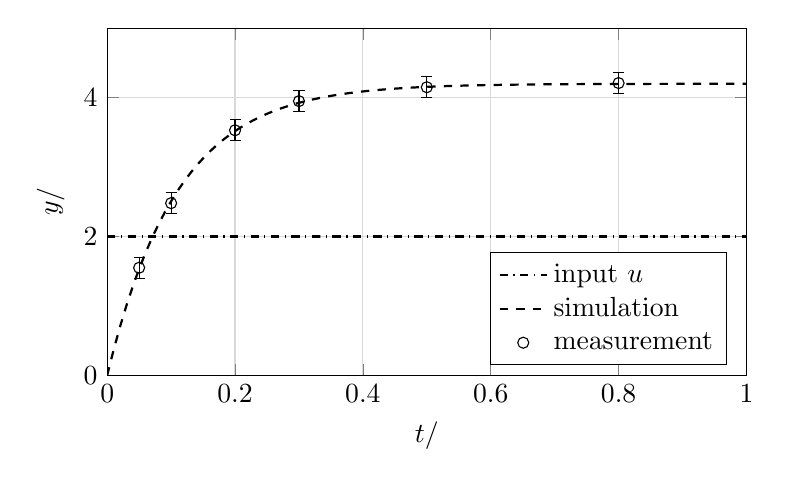
\begin{tikzpicture}
    \begin{axis}[
        width=0.8\textwidth, height=0.494\textwidth,
        xlabel={$t$/\unit{\second}}, ylabel={$y$/\unit{\volt}},
        xmin=0, xmax=1, ymin=0, ymax=5,
        grid=major, grid style={gray!30},
        legend pos=south east, legend cell align=left,
        /pgf/number format/.cd, use period,
      ]
      % Eingangssprung: strichpunktiert
      \addplot[black, dashdotted, thick, domain=0:1] {2};
      \addlegendentry{input $u$}
      % Modell: Strichlinie
      \addplot[black, dashed, thick, domain=0:1, samples=100]
        {4.2*(1-exp(-x/0.11))};
      \addlegendentry{simulation}
      % Messpunkte mit Fehlerbalken: nur Marker, keine Linie
      \addplot[black, only marks, mark=o,
               error bars/.cd, y dir=both, y explicit]
        coordinates {
          (0.05,1.55) +- (0,0.15)
          (0.10,2.48) +- (0,0.15)
          (0.20,3.53) +- (0,0.15)
          (0.30,3.95) +- (0,0.15)
          (0.50,4.15) +- (0,0.15)
          (0.80,4.21) +- (0,0.15)
        };
      \addlegendentry{measurement}
    \end{axis}
  \end{tikzpicture}
  \caption[Measured and simulated step response]{Comparison of measured
    (circles with error bars) and simulated (dashed) step response of the DC
    motor for an input step of \qty{2}{\volt} (dash-dotted)}
  \label{fig:plot}
\end{figure}
%<<<

\section{Diagram from MATLAB}
The export code is given as a comment in the source file.
%>>> MATLAB-Export als Vektorgrafik (M061, M065, M068), Code als Kommentar:
%  plot(t, y, 'k-', t, ym, 'k--');            % schwarz, Linienarten statt Farben
%  xlabel('$t$/s', 'Interpreter','latex');    % Größe/Einheit, keine [ ]
%  ylabel('$y$/V', 'Interpreter','latex');
%  legend('measurement', 'simulation');       % kein title(...)!
%  set(gcf, 'Units','centimeters', 'Position',[0 0 12 7.4]);   % 1.618 : 1
%  exportgraphics(gcf, 'img/step_response.pdf', 'ContentType','vector');
% Danach in LaTeX:
%  \includegraphics[width=0.8\textwidth]{img/step_response}
%<<<

% #####################################################################
\chapter{Citations and Quotations}
% #####################################################################

\section{Citing (M069–M071, M108)}
%>>> \cite direkt hinter der übernommenen Aussage, vor dem Satzpunkt
The step response method was originally proposed by Ziegler and Nichols and
later revisited~\cite{astrom2004}. Several sources can be cited at
once~\cite{lunze2020, skript}. The motor data are taken from the
datasheet~\cite{datenblatt}.
%<<<

%>>> Ganzer Absatz sinngemäß übernommen: am Anfang kennzeichnen (M108)
The following paragraph is based on~\cite{lunze2020}. A first-order lag
element responds to a step input with an exponential approach to its final
value. After one time constant, \qty{63.2}{\percent} of the final value is
reached.
%<<<

\section{Short Literal Quotation (M074)}
%>>> Im Fließtext, in Anführungszeichen, kursiv (sparsam verwenden, M073)
According to the datasheet, the motor is \enquote{\textit{designed for
continuous operation}}~\cite{datenblatt}.
%<<<

\section{Long Literal Quotation (M075)}
%>>> Eigener Absatz, eingerückt, geringerer Zeilenabstand
\begin{displayquote}
  \setstretch{1.0}
  The controller parameters [of the PID controller] are obtained directly
  from the step response [\dots] and are therefore easy to apply in
  practice.~\cite{astrom2004}
\end{displayquote}
%<<<

\section{Online Source (M081)}
%>>> Nur in Ausnahmefällen; im .bib unbedingt url + urldate angeben
The figure was exported with the function \texttt{exportgraphics}~\cite{matlabdoc}.
%<<<

% #####################################################################
\chapter{List of Symbols}
% #####################################################################
%>>> Formelzeichenverzeichnis (M049): Einheit, bei Konstanten Wert;
%    keine Indizes einzeln, keine Operatoren (Delta, Sigma), kein pi, e
\begin{tabularx}{\textwidth}{l X l}
  \toprule
  Symbol & Description & Unit \\
  \midrule
  $K$ & static gain & \unit{\volt\per\volt} \\
  $T$ & time constant & \unit{\second} \\
  $t$ & time & \unit{\second} \\
  $u$ & input voltage & \unit{\volt} \\
  $y$ & output voltage & \unit{\volt} \\
  $\omega$ & angular velocity & \unit{\radian\per\second} \\
  $g$ & gravitational acceleration, \qty{9.81}{\metre\per\second\squared} & \unit{\metre\per\second\squared} \\
  \bottomrule
\end{tabularx}
%<<<

% #####################################################################
\chapter{Code Listing}
% #####################################################################
%>>> Programmcode (listings ist in der Klasse geladen)
\begin{lstlisting}[language=Matlab, caption={Identification of the time constant}]
y63 = 0.632 * y_end;          % 63.2 % of the final value
T   = t(find(y >= y63, 1));   % first sample above threshold
\end{lstlisting}
%<<<

\printbibliography[heading=bibintoc]

\end{document}
